%%%%%%%%%%%%%%%%%%%%%%%%%%%%%%%%%%%%%%%%%
% Short Sectioned Assignment
% LaTeX Template
% Version 1.0 (5/5/12)
%
% This template has been downloaded from:
% http://www.LaTeXTemplates.com
%
% Original author:
% Frits Wenneker (http://www.howtotex.com)
%
% License:
% CC BY-NC-SA 3.0 (http://creativecommons.org/licenses/by-nc-sa/3.0/)
%
%%%%%%%%%%%%%%%%%%%%%%%%%%%%%%%%%%%%%%%%%

%----------------------------------------------------------------------------------------
%	PACKAGES AND OTHER DOCUMENT CONFIGURATIONS
%----------------------------------------------------------------------------------------

\documentclass[paper=a4, fontsize=11pt]{scrartcl} % A4 paper and 11pt font size

\usepackage[T1]{fontenc} % Use 8-bit encoding that has 256 glyphs
\usepackage[swedish, english]{babel} % English language/hyphenation
\usepackage{sectsty} % Allows customizing section commands

\usepackage{graphicx}

\usepackage{hyperref}

\allsectionsfont{\normalfont\scshape} % Make all sections centered, the default font and small caps
\sectionfont{\center \normalfont\scshape}

\usepackage{fancyhdr} % Custom headers and footers
\pagestyle{fancyplain} % Makes all pages in the document conform to the custom headers and footers
\fancyhead{} % No page header - if you want one, create it in the same way as the footers below
\fancyfoot[L]{} % Empty left footer
\fancyfoot[C]{} % Empty center footer
\fancyfoot[R]{\thepage} % Page numbering for right footer
\renewcommand{\headrulewidth}{0pt} % Remove header underlines
\renewcommand{\footrulewidth}{0pt} % Remove footer underlines

\setlength{\headheight}{13.6pt} % Customize the height of the header
\setlength\parindent{0pt} % Removes all indentation from paragraphs - comment this line for an assignment with lots of text

%----------------------------------------------------------------------------------------
%	TITLE SECTION
%----------------------------------------------------------------------------------------

\newcommand{\horrule}[1]{\rule{\linewidth}{#1}} % Create horizontal rule command with 1 argument of height

\title{	
\normalfont \normalsize 
\textsc{Lule� Tekniska Universitet} \\ [25pt] % Your university, school and/or department name(s)
\horrule{1pt} \\[0.4cm] % top horizontal rule
\huge Sprints \\ % The assignment title
\horrule{1pt} \\[0.5cm] % bottom horizontal rule
}

\author{Victor Persson,\\ Niklas Eliasson} % Your name

\date{\normalsize\today} % Today's date or a custom date

\begin{document}

\maketitle % Print the title

%----------------------------------------------------------------------------------------

\section{}

%------------------------------------------------

%\subsection{Summary}

\subsection{User stories}
	Anv�ndare
	\begin{itemize}
		\item Butiksadministrat�r
		\begin{itemize}
			\item r/w priser
			\item r/w kampanjer
			\item r/w lagerstatus
			\item r/w kategorier
			\item r leveransstatus
			\item r kundinfo
		\end{itemize}
		\item Lagerarbetare
		\begin{itemize}
			\item r/w lagerstatus
			\item r/w leveransstatus
			\item r kundinfo
		\end{itemize}
		\item Inloggad kund
		\begin{itemize}
			\item r/w sin egen kontaktinformation
			\item l�sa sin egen orderhistorik
			\item l�sa sortimentet (produkter, priser, kampanjer, lagerstatus)
			\item l�gga ordrar
			\item ? Spara/skicka kundkorg
		\end{itemize}
		\item Ej inloggad kund
		\begin{itemize}
			\item l�sa sortimentet (produkter, priser, kampanjer, lagerstatus)
			\item l�gga ordrar
			\item ? skicka kundkorg (e-post)
		\end{itemize}

	See Figure \ref{fig:1} - \ref{fig:4}

	\begin{figure}
		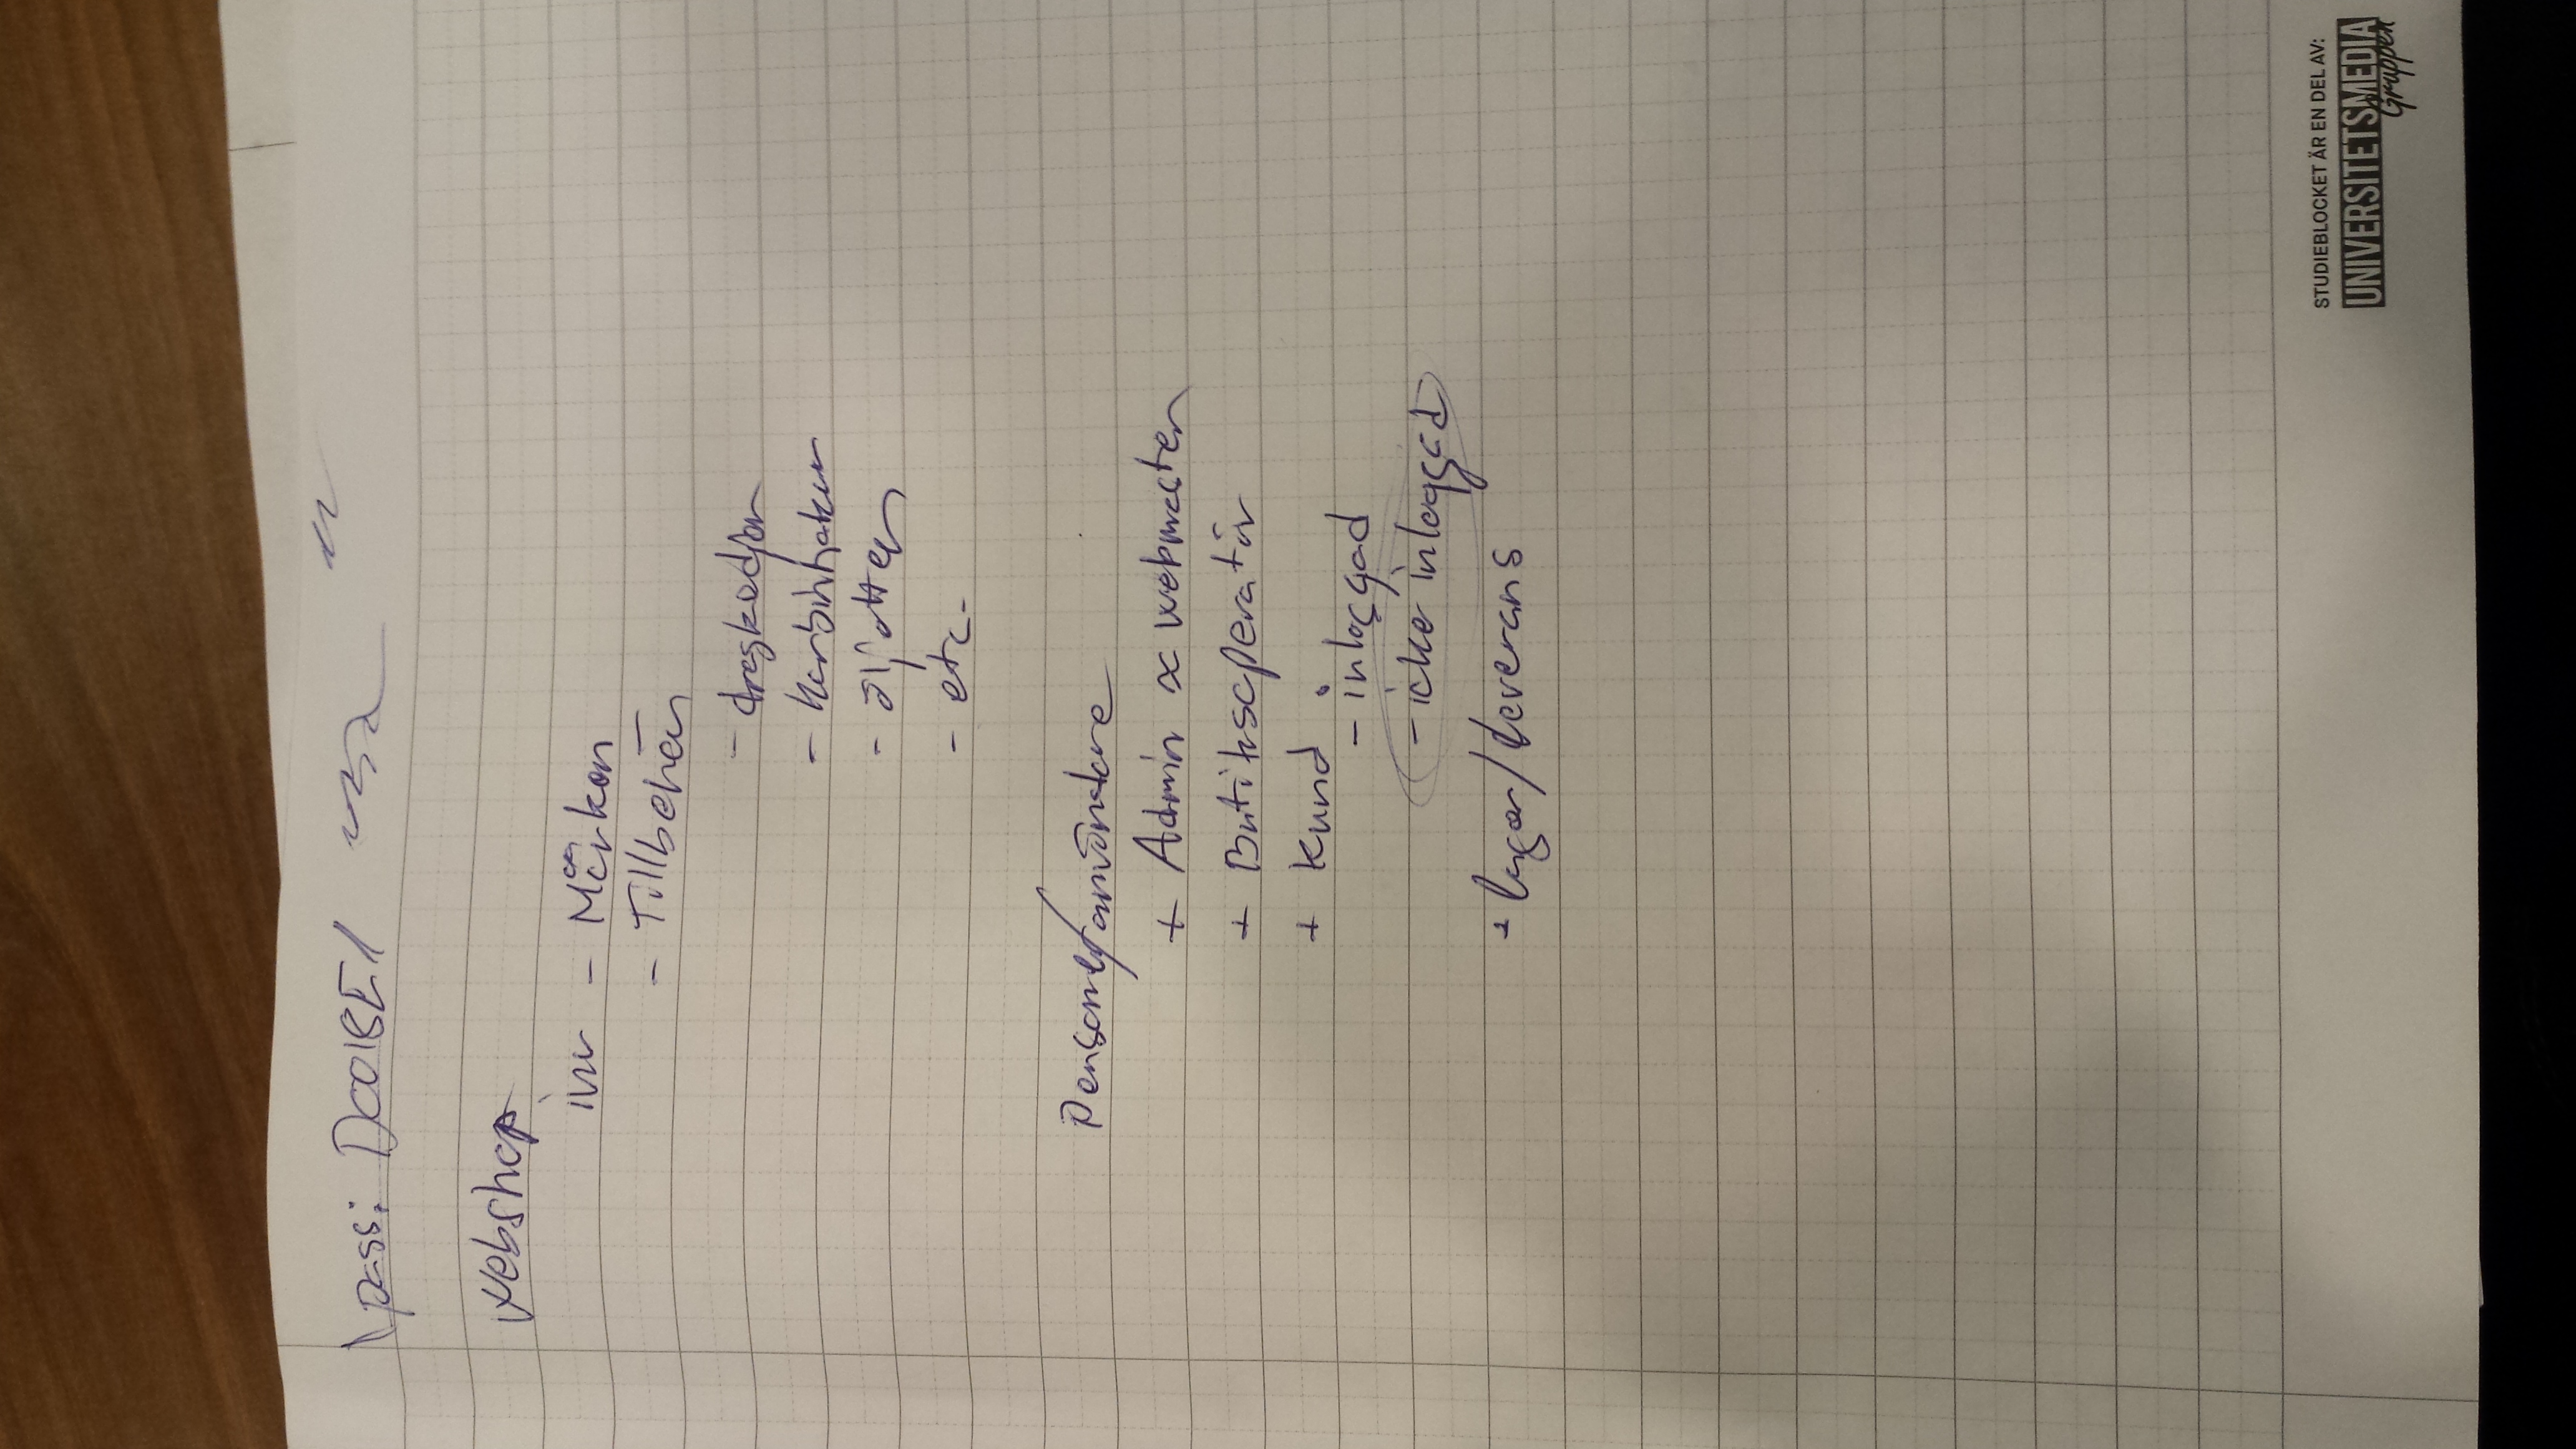
\includegraphics[scale=0.12]{artifacts/Inventory+Users.jpeg}
		\caption{}
		\label{fig:1}
	\end{figure}
	
	\begin{figure}
		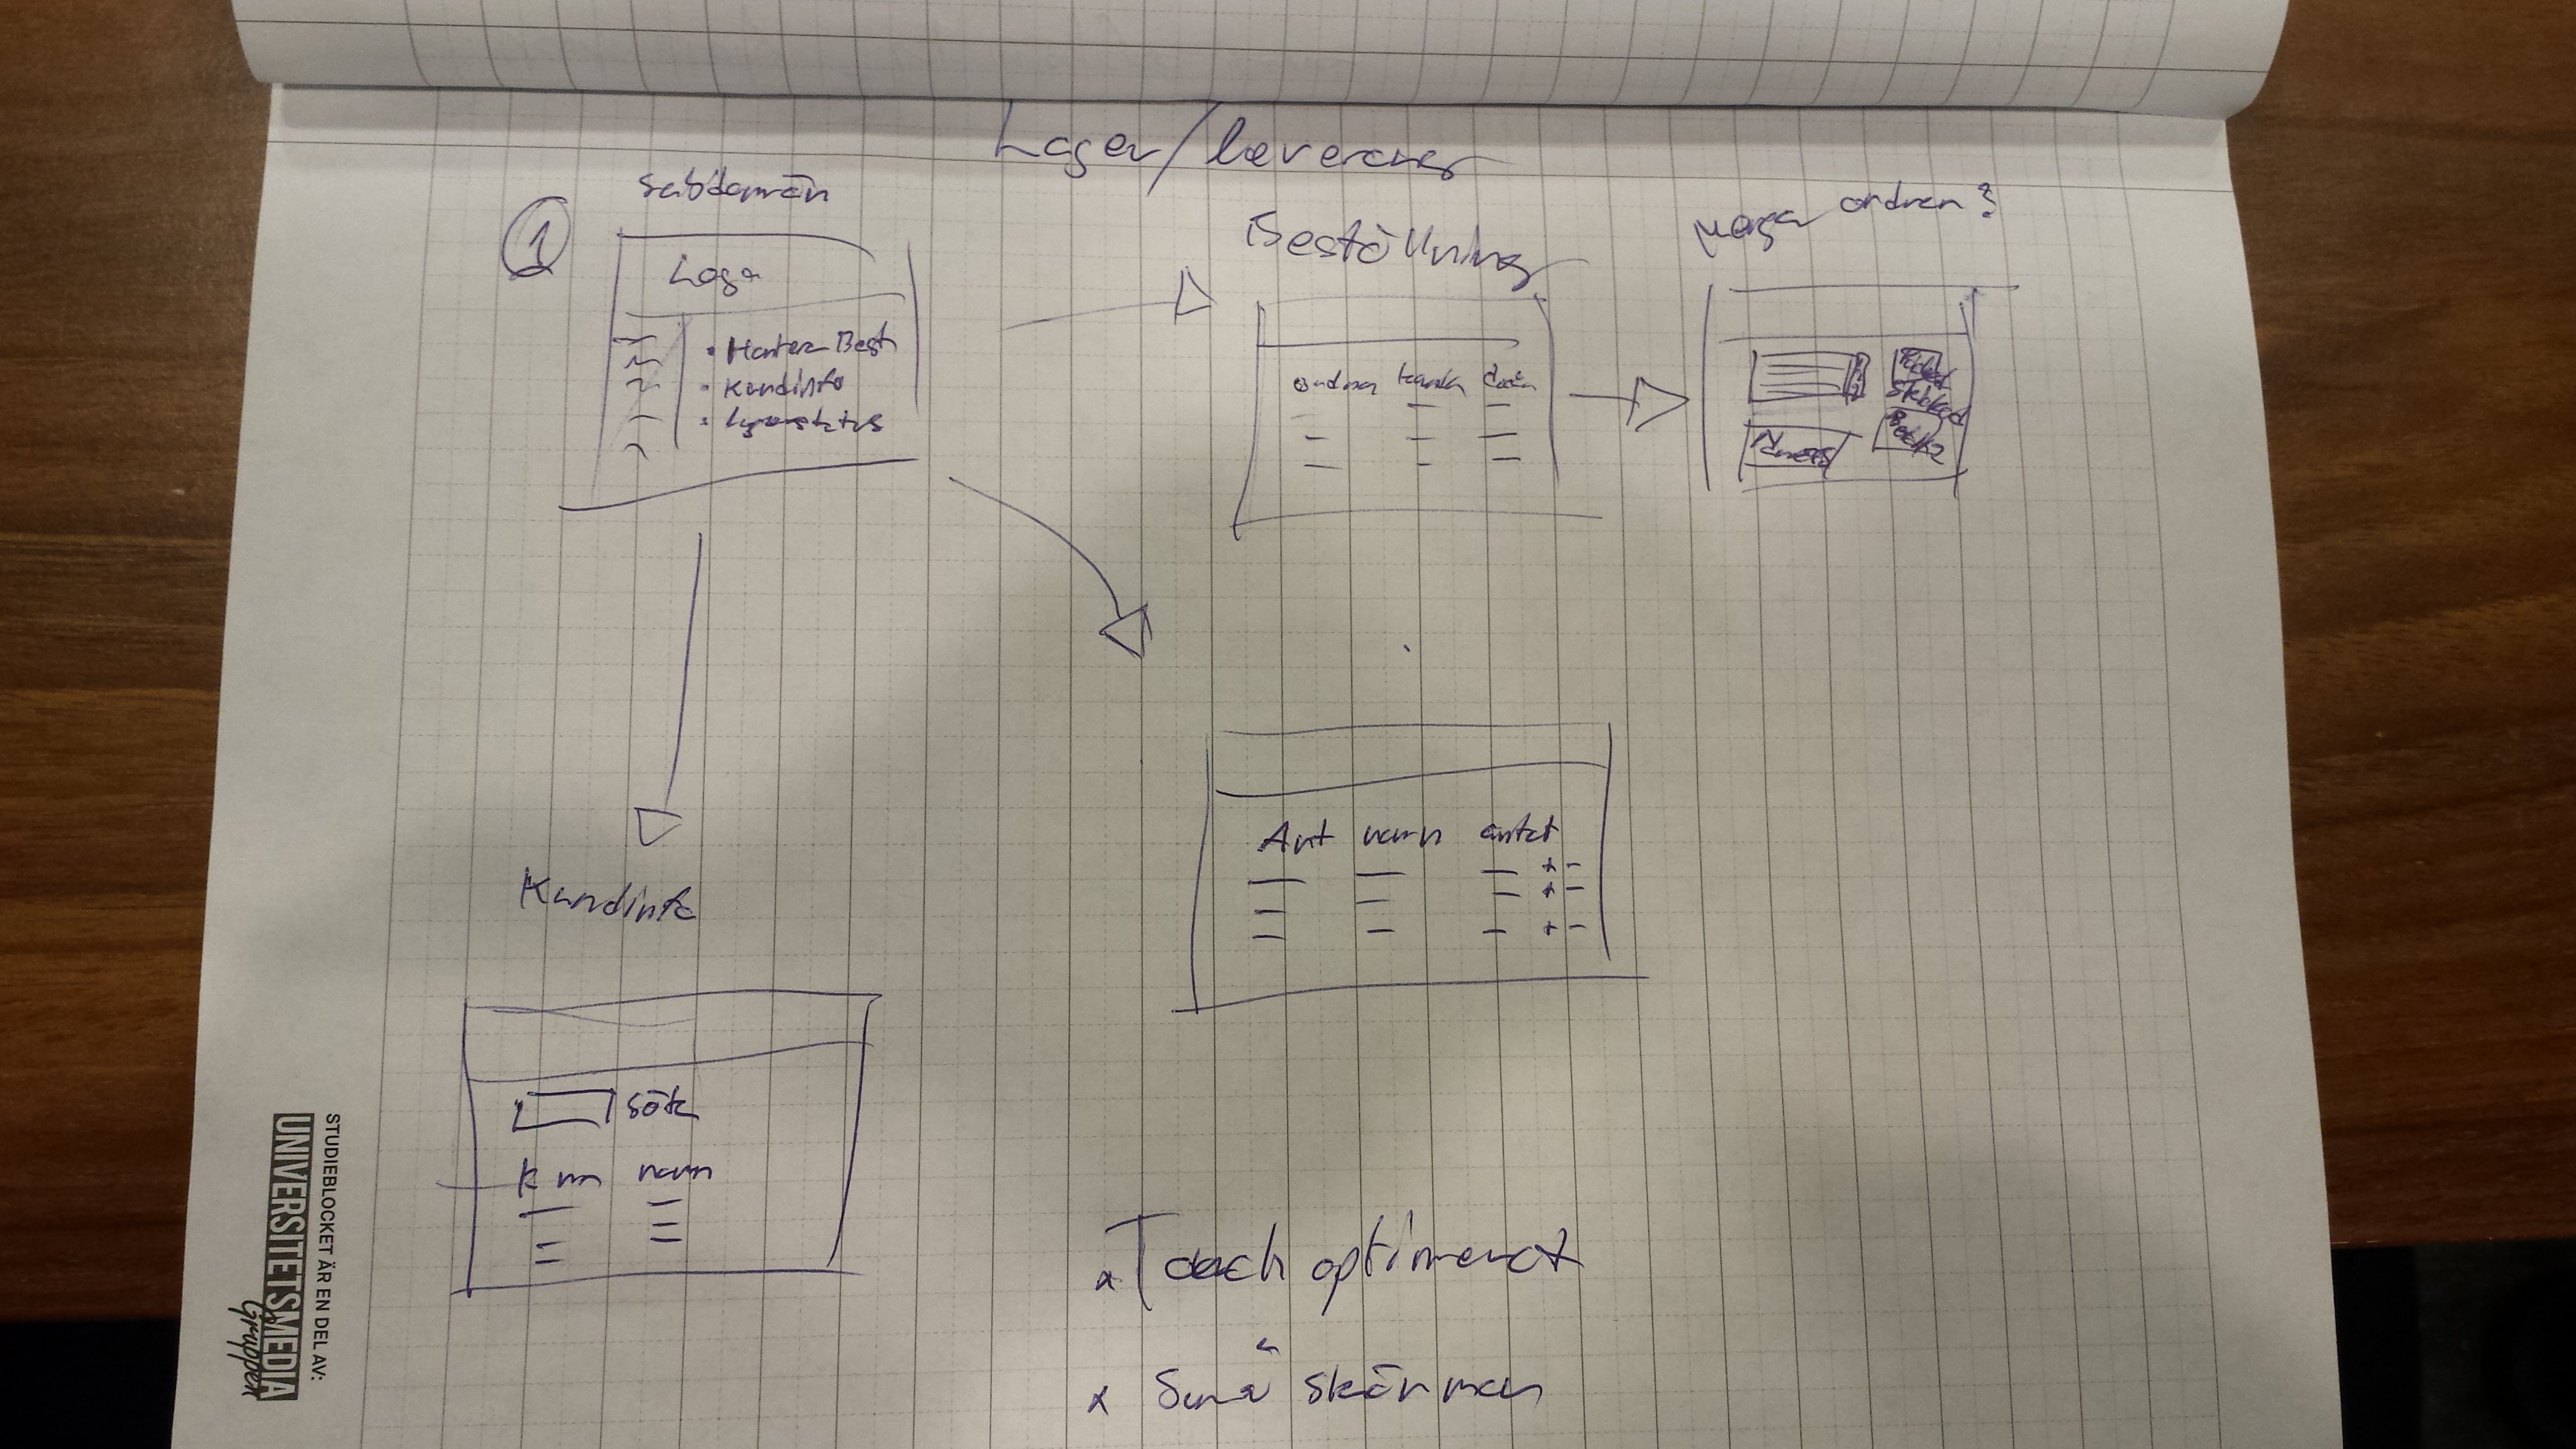
\includegraphics[scale=0.12]{artifacts/Lager.jpeg}
		\caption{}
		\label{fig:2}
	\end{figure}

	\begin{figure}
		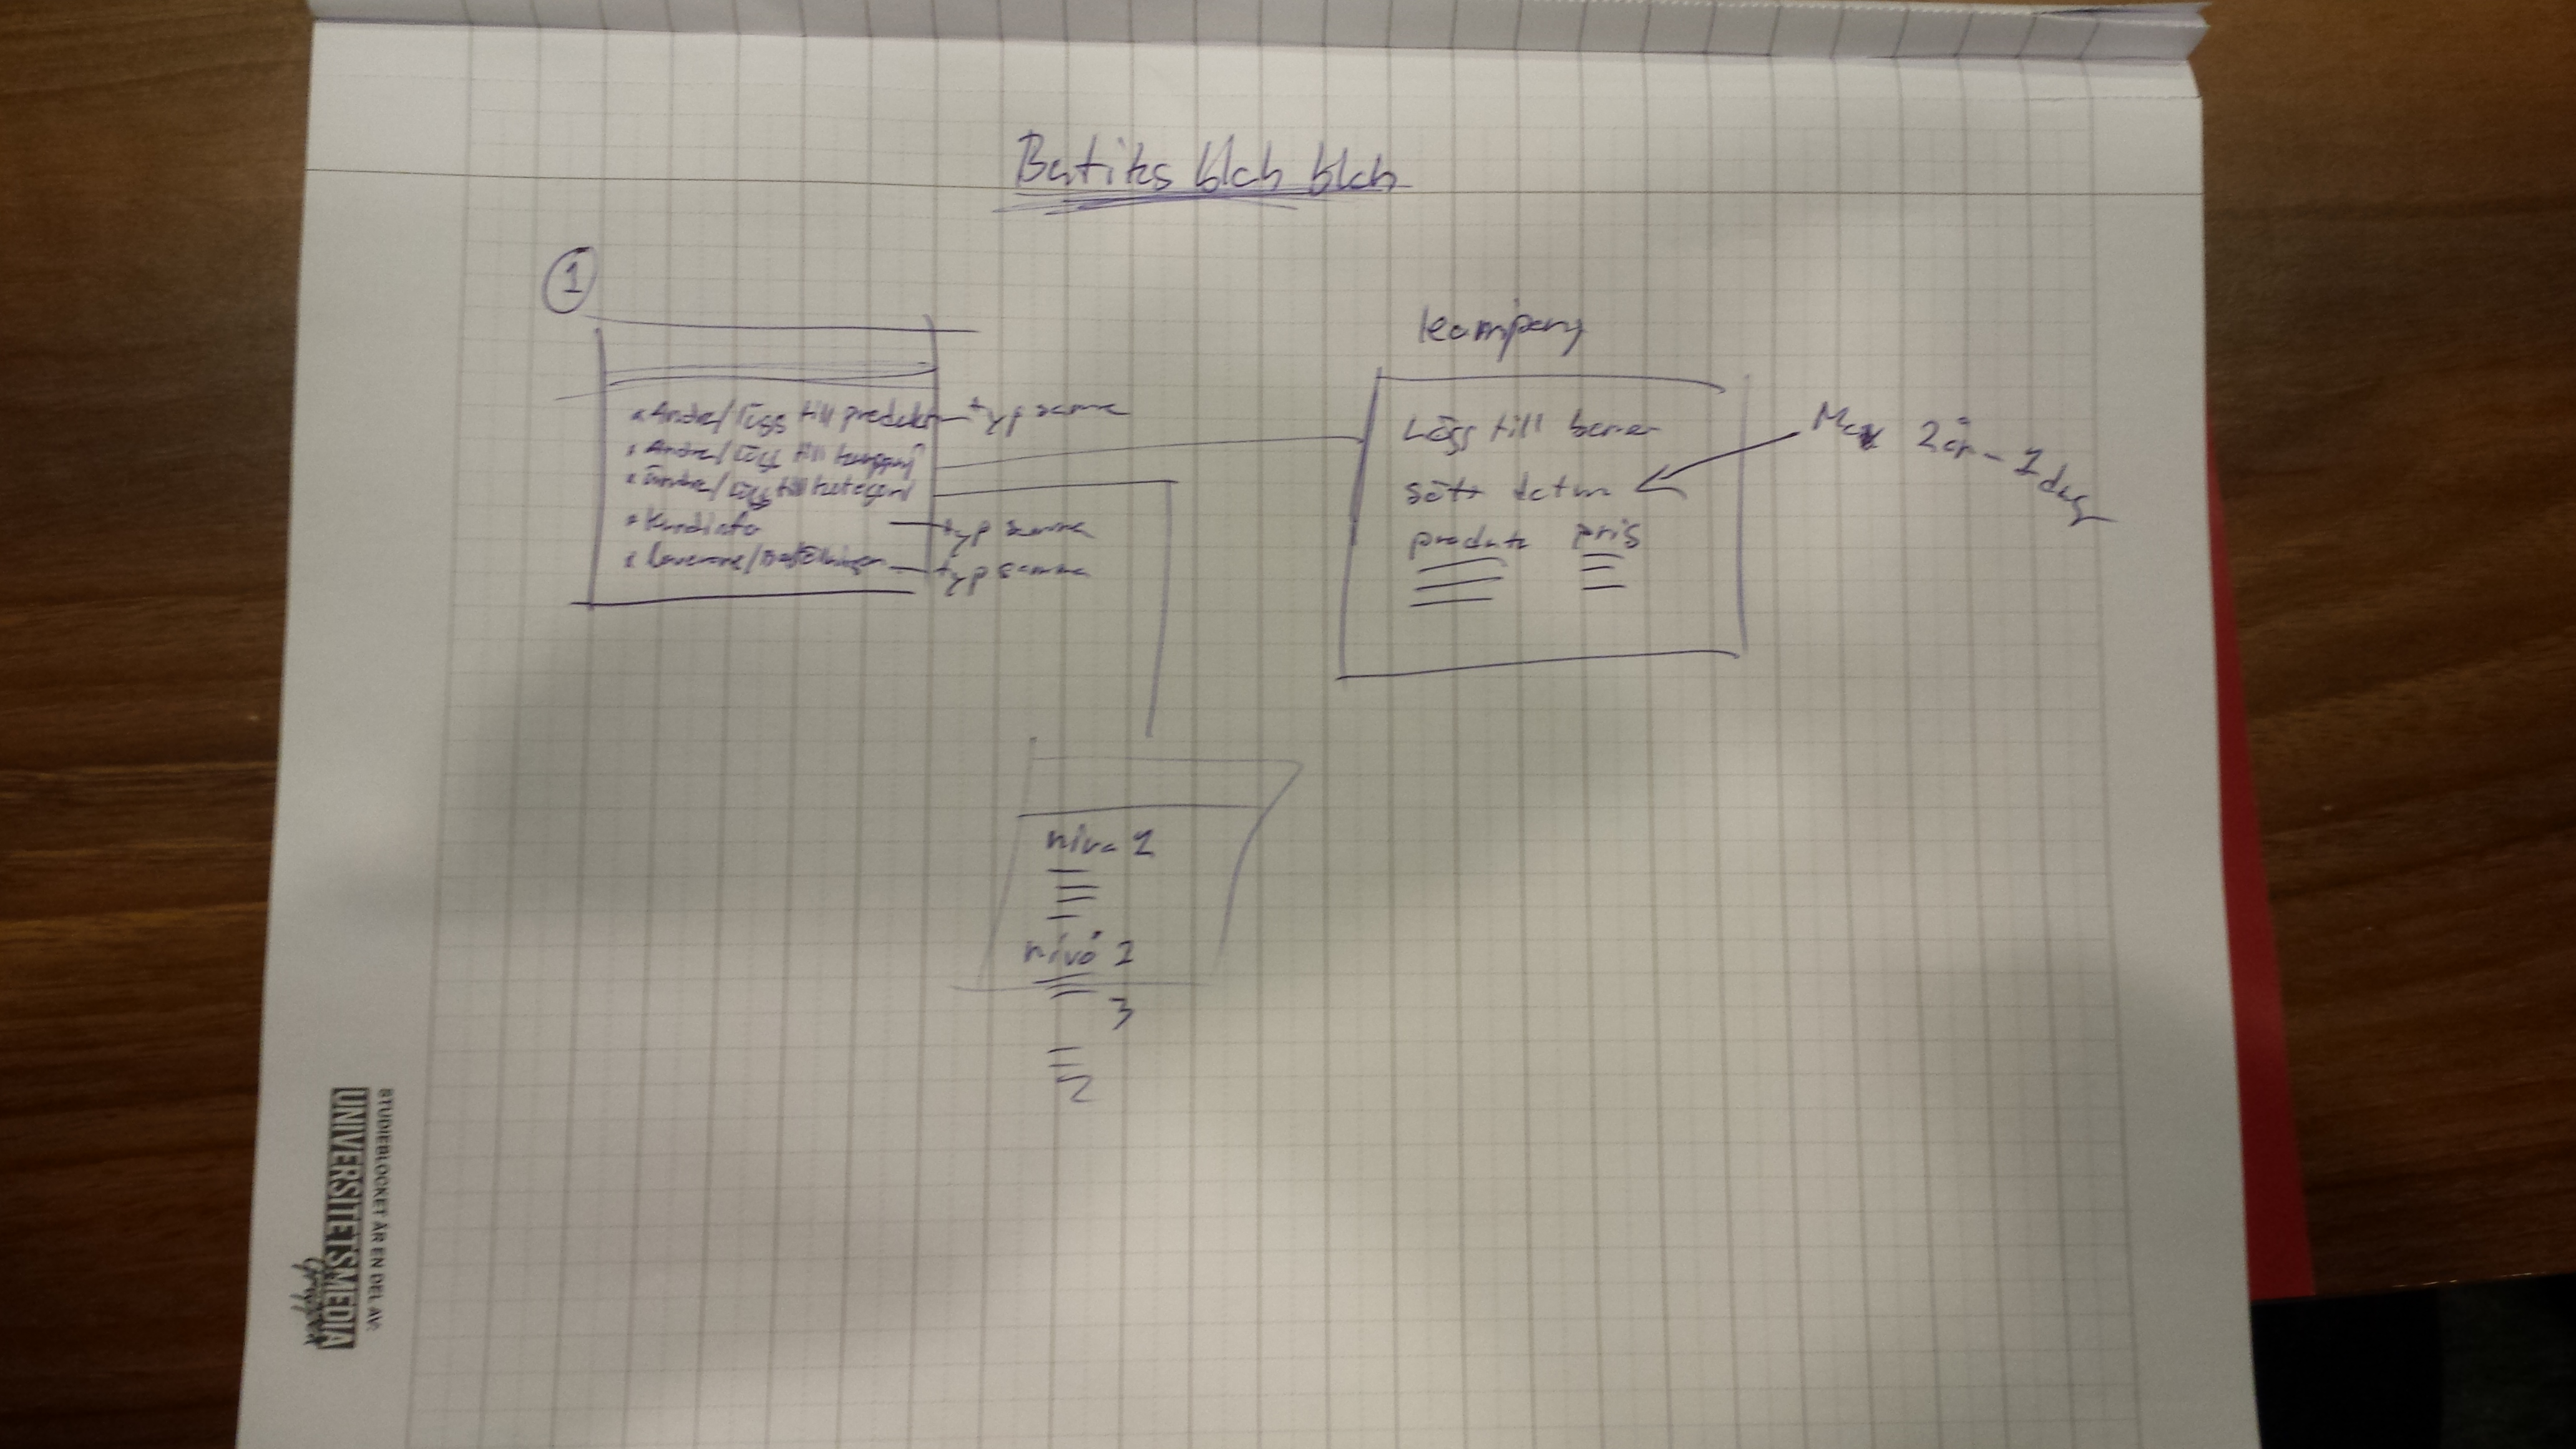
\includegraphics[scale=0.12]{artifacts/ButiksAdmin.jpeg}
		\caption{}
		\label{fig:3}
	\end{figure}

	\begin{figure}
		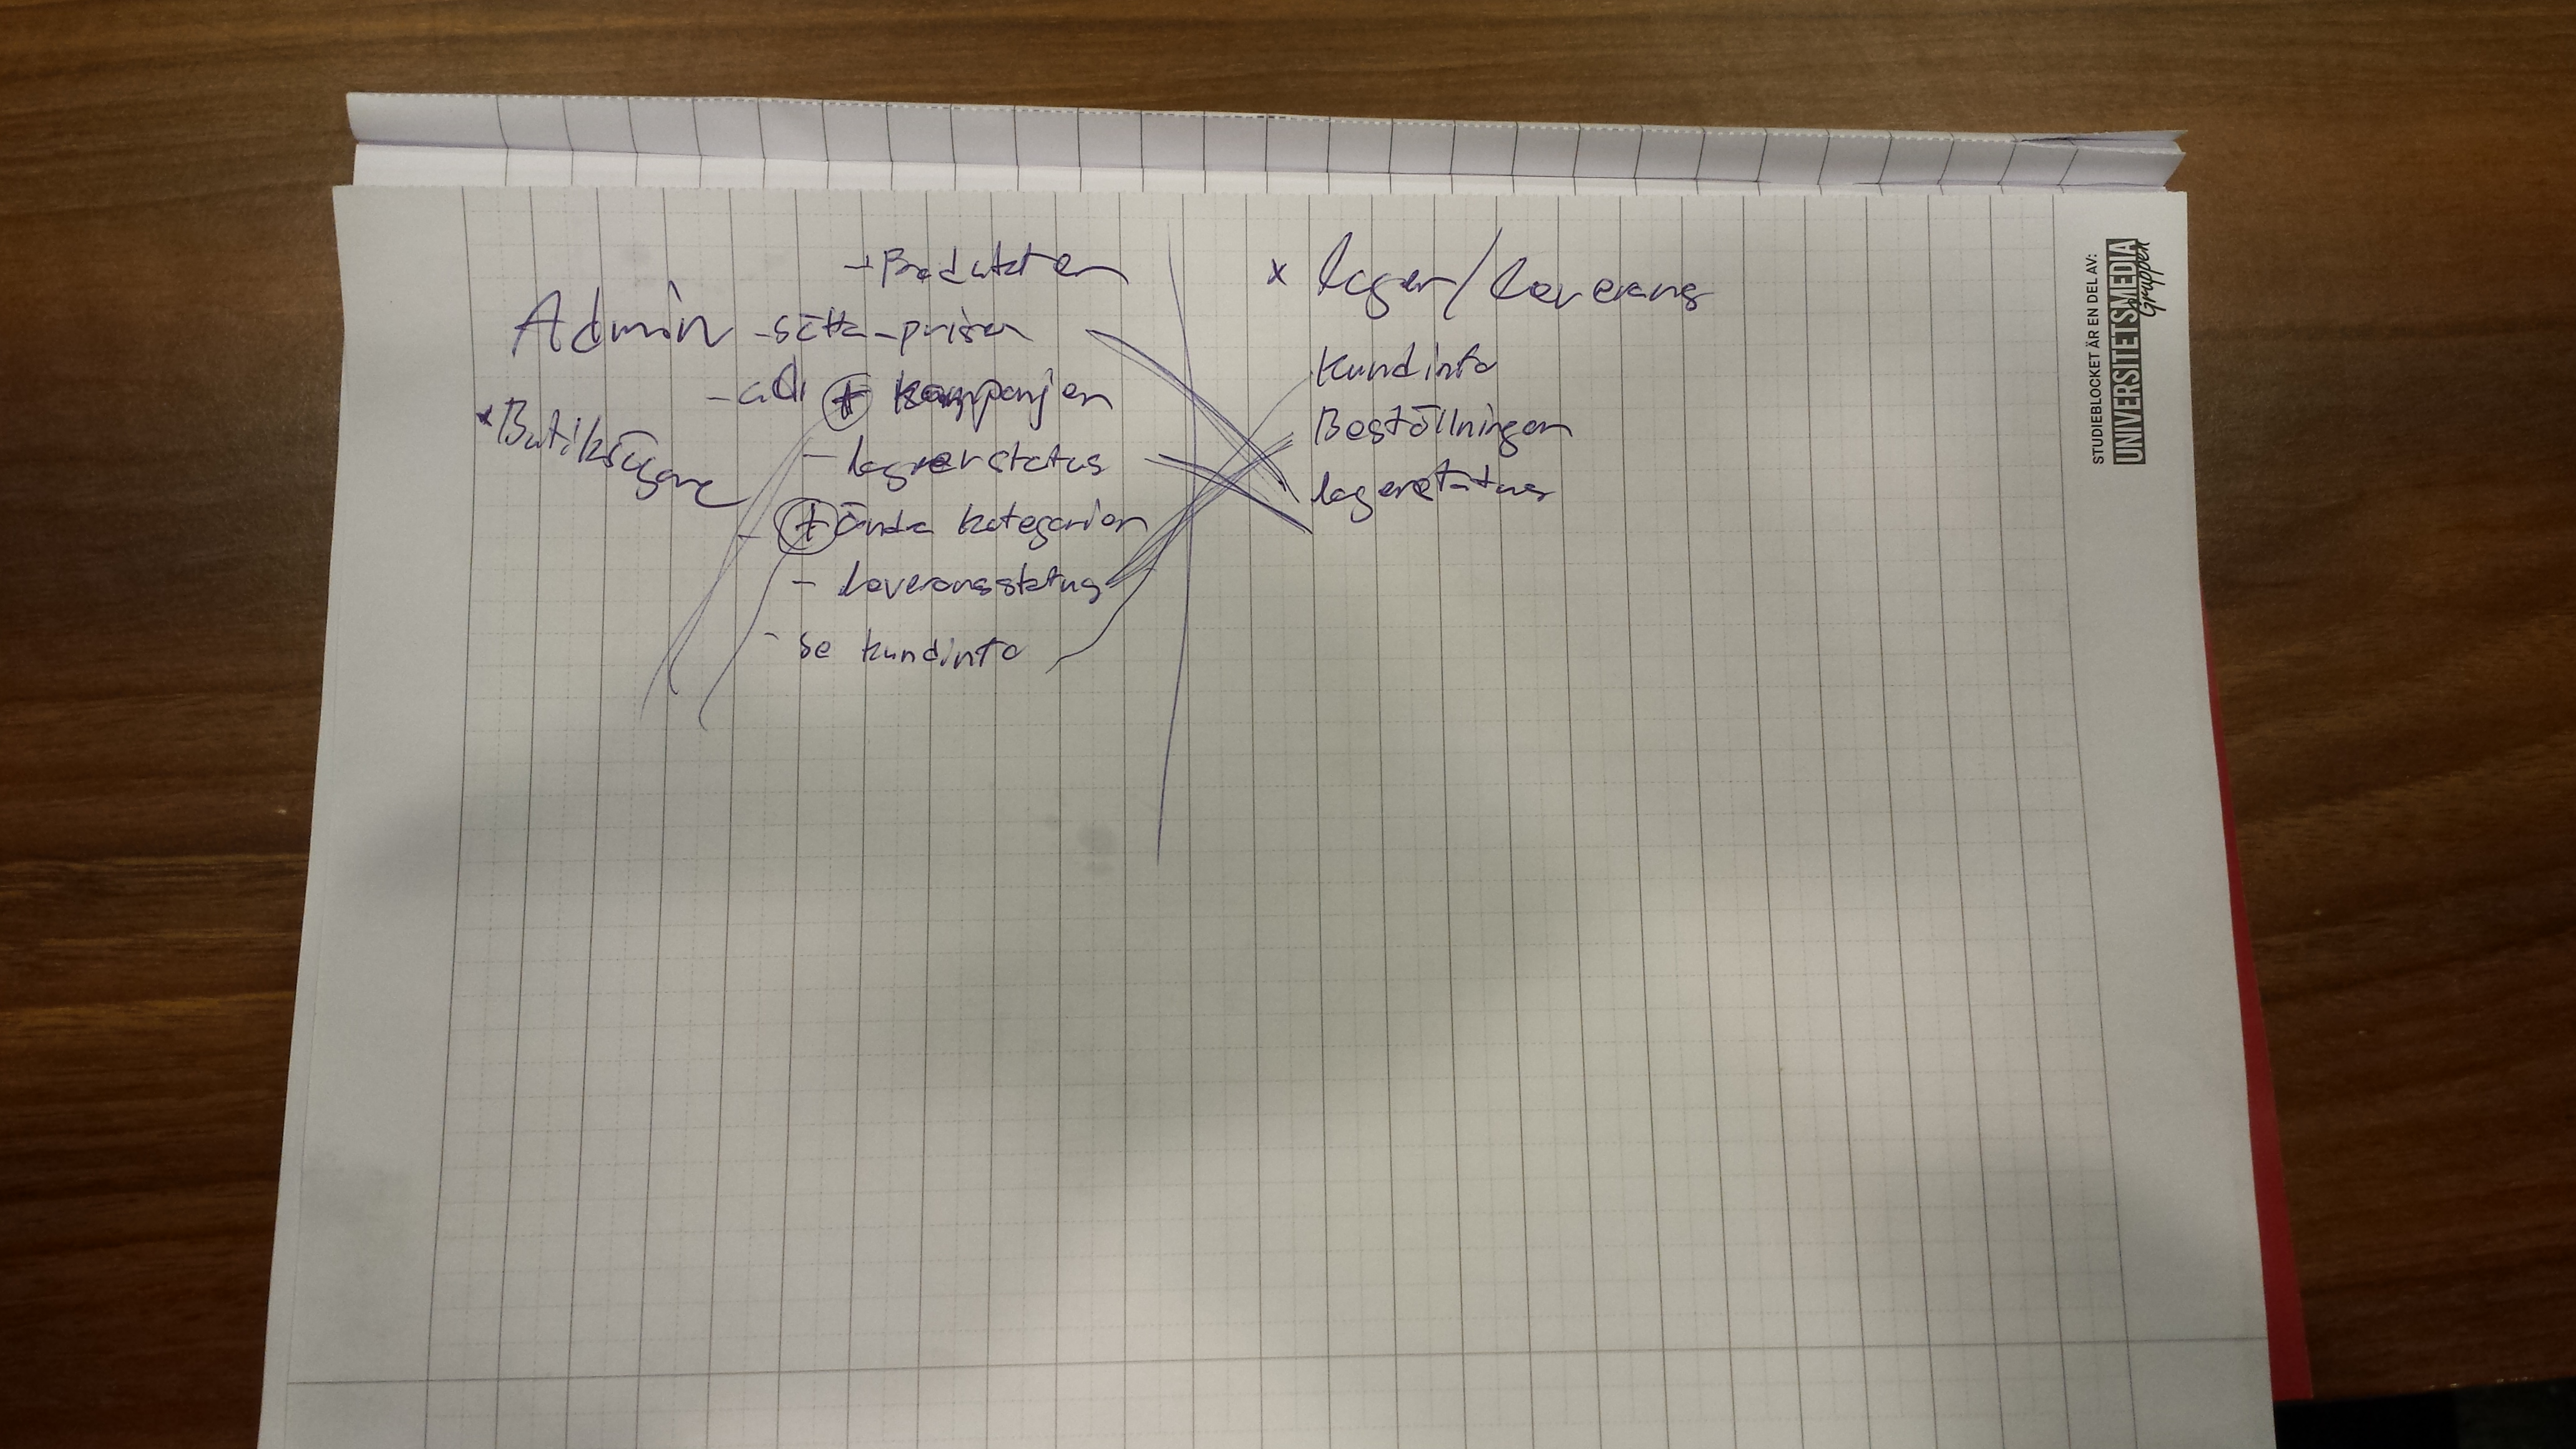
\includegraphics[scale=0.12]{artifacts/Admin.jpeg}
		\caption{}
		\label{fig:4}
	\end{figure}

\subsection{System architecture}
	During development we run the system on Ruby on Rails (RoR) built in web server
	Puma and sqlight3 for simplicity, but intend to move to a MariaDB database
	and a NGINX webserver with Phusion Passenger for RoR. We host
	the servers ourselves because it seemed seemed fun, educational and fairly simple. 

\subsection{Backlog} 
	\begin{tabular}{|l|l|l|l|l|}
		\hline
		\# & Title & Priority & Time est. & Description \\ \hline
		301 & Startsida & 100 & 2 & \\ \hline
		302 & Dynamisk meny fr�n kategorier & 90 & 2 & \\ \hline
		304 & Produktsida & 110 & 4 & \\ \hline
		305 & Kundkorg & 80 & 8 & \\ \hline
		306 & Betalsida & 5 & 12 & \\ \hline
		307 & Profilsida (kundkort) & 45 & 2 & \\ \hline
		308 & Orderhistorik & 45 & 1 & \\ \hline
		309 & Kundinlogg & 50 & 2 & \\ \hline
		310 & Registrering & 60 & 4 & \\ \hline
		311 & Produkts�kning & 45 & 1 & \\ \hline
		400 & Backendinloggning & 25 & 2 & \\ \hline
		401 & Backendinterface & 10 & 2 & \\ \hline
		403 & Kategorisida & 35 & 4 & \\ \hline
		407 & Kundinformation & 25 & 1 & \\ \hline
		410 & Kampanjhantering & 10 & 3 & \\ \hline
		1 & Personnummer -/+ hantering & 5 & 1 & \\ \hline
	\end{tabular}

	Planing is done at Trello.com
	\url{https://trello.com/b/JxDCHBcm}

\subsection{Database schema}	
	See Figure \ref{fig:6}
	\begin{figure}
		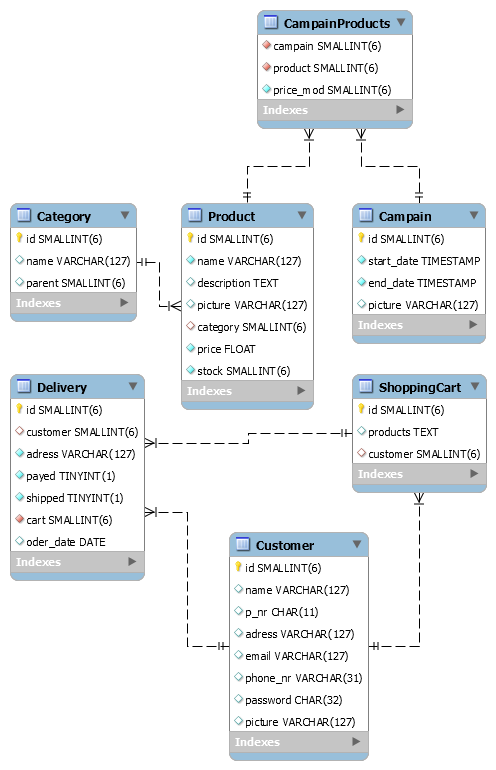
\includegraphics[scale=0.7]{artifacts/db_implemented_1_1.png}
		\caption{Database design.}
		\label{fig:6}
	\end{figure}

\subsection{Code}
	All code is avalible at github.
	\url{https://github.com/nikalas/D0018E-Databasteknik.git}

%\subsection{Test case specifications}

\subsection{Limitations and improvements}

	We decided to put off saving payment methods and/or information. Might end
	up readding it to the backlog if it looks like we will have time to spare. 

\end{document}
